\documentclass[12pt]{article}
\usepackage{preamble}
\usepackage{longtable}
\usepackage{mathtext}
\usepackage[T2A]{fontenc}
\usepackage[utf8]{inputenc}
\usepackage{mathtools}
\usepackage{pythonhighlight}
\usepackage{nccmath}
\usepackage[russian]{babel}
\newenvironment{system}%
{\left\lbrace\begin{array}{@{}l@{}}}%
{\end{array}\right.}

\geometry{a4paper, left=2.5cm, right=2.5cm, top=2cm, bottom=2.5cm}

\pagestyle{plain}

\newcommand{\placeholder}[1]{{\color{magenta}#1}}

\chead{
    \begin{minipage}{1\linewidth}
        \begin{wrapfigure}{r}{0pt}
            
\includegraphics[height=1cm]{images/logo}
        \end{wrapfigure}
        {
            \centering
            \sffamily\scriptsize
            \textbf{
                Санкт-Петербургский национальный исследовательский университет \\
                информационных технологий, механики и оптики}
            %th3p4g
            \vspace{2mm}

            \quad\quad\quad\quad\quad\quad\ \textbf{УЧЕБНЫЙ ЦЕНТР ОБЩЕЙ ФИЗИКИ ФТФ}
        }
    \end{minipage}
}



\begin{document}
    \vspace*{2\baselineskip}

    \thispagestyle{fancy}

    \noindent
    \textbf{Группа} \underline{M3200} \hfill \textbf{К работе допущен} \underline{\hspace{4cm}} \\[0.5cm]
    \textbf{Студент} \underline{Насонов Пётр Алексеевич} \hfill \textbf{Работа выполнена} \underline{\hspace{4cm}} \\[0.5cm]
    \textbf{Преподаватель} \underline{Хвастунов Н. Н.} \hfill \textbf{Отчет принят} \underline{\hspace{4.85cm}} \\


    \begin{center}
    {\huge \textbf{Численное моделирование по физике. Электростатика}}

        \smallvspace

    \end{center}

    \begin{center}
        {\large \textbf{Условия. Частица в конденсаторе}} \\
    \end{center}

    Электрон влетает в цилиндрический конденсатор с начальной скоростью V, посередине между
обкладками, параллельно образующим цилиндра. При какой минимальной разности потенциалов,
приложенной к обкладкам, электрон не успеет вылететь из конденсатора. Краевыми эффектами
пренебречь.
Построить графики зависимости $ y(x), V_y(t), a_y(t), y(t)$. Координатные оси направлены как показано
на рисунке.
Рассчитать время полета t и конечную скорость электрона $V_\text{кон}$

    \large \textbf{Используемые константы} \normalsize

    Вариант 11.

    \normalsize
    \begin{enumerate}
        \item Радиус внутренней обкладки $R_1$ = 0.06 м
        \item Радиус внешней обкладки $R_2$ = 0.13 м
        \item Изначальная скорость электрона $V$ = $3.5 \cdot 10^6 \frac{\text{м}}{\text{с}}$
        \item Длина конденсатора $L$ = 0.21 м
        \item Масса электрона $m_e$ = $9.1 \cdot 10^{-31}$ кг
        \item  Заряд электрона $q_e$ = $1.6 \cdot 10^{-16}$ Кл
    \end{enumerate}
    

\large \textbf{Решение} \normalsize

Чтобы электрон не вылететь из конденсатора, то он должен столкнуться с одной из обкладок. Пусть $t_0$ - время полета электрона до столкновения.
    В задаче стоит вопрос про минимальную разность потенциалов, при которой электрон не вылетит из конденсатора. Позже в задаче мы придем
    к тому что разность потенциалов прямопрорционально зависит от скорости электрона и времени его столкновения. Таким образом, если 
    разность потенциалов будет меньше нуля, то о минимальной говорить в этом контексте не совсем корректно. Поэтому
    будем искать для случая когда разность потенциалов положительна. Если это так, то линии напряженности направлены из центра перпендикулярно оси
    обкладок. Т.е. стокнется с внешней обкладкой. 


    Т.к. у нас цилиндрический конденсатор:

    $$E = \frac{2kq}{Lr} \text{(в нашем случае $r$ = $y$)}$$ 

    $$q = \frac{\Delta \varphi L}{2k \ln \frac{R_2}{R_1}}$$ 

    И таким образом получаем:

    $$E(y) = \frac{\Delta \varphi }{y \ln \frac{R_2}{R_1}}$$

    Чтобы сделать графики и в целом решать нашу задачу нам нужно только найти функцию укорения:

    $$a_y(y) = \frac{F}{m_e} = \frac{q_e E(y)}{m_e} = \frac{q_e \Delta \varphi }{m_e y \ln \frac{R_2}{R_1}}$$

    \begin{equation}
        \begin{system}
        \frac{d^2y}{dt^2} = \frac{q_e \Delta \varphi }{m_e y \ln \frac{R_2}{R_1}} \\
        y(t_0) = R_2 \\
        y(0) = \frac{R_1+R_2}{2} \\
        V \cdot t_0 = L \\
        V_y(0)=0 \\
        \end{system}
    \end{equation}

    Тут можно конечно применить математическую магию и решать этот дифур самому, на я воспользуюсь scipy из python:

    \large \textbf{Загоняя дифур в питон:} \normalsize

    \begin{python}
sol = solve_ivp(equations, t_span, y0_v0, t_eval=t_eval)

t = sol.t
y = sol.y[0]
v_y = sol.y[1]

#equations is acceleration function))
def equations(t, yv):
    y, v_y = yv
    a_y = q_e * Delta_phi / (m_e * y * log_R)
    return [v_y, a_y]
\end{python}

Со временем все просто - чем дольше летим тем меньше можем сделать разность потенциалов.
Однако саму разность потенциалов надо найти численно. Для этого воспользуемся методом бинарного поиска. Критерий будет банален - 
если мы к концу времени улетели слишком далеко за наш конденсатор, то значит что слишком быстро летели. Значит можно разность 
потенциалов сделать меньше. И наоборот.
И получаем все что нам надо:\\

$\Delta \varphi = 8.600117$ Вольт\\
Время полета $6 \cdot 10^{-8}$ с\\
$V_\text{кон}: 1.1076 \cdot 10^{6} \frac{\text{м}}{\text{с}}$\\

Получаем такие графики:

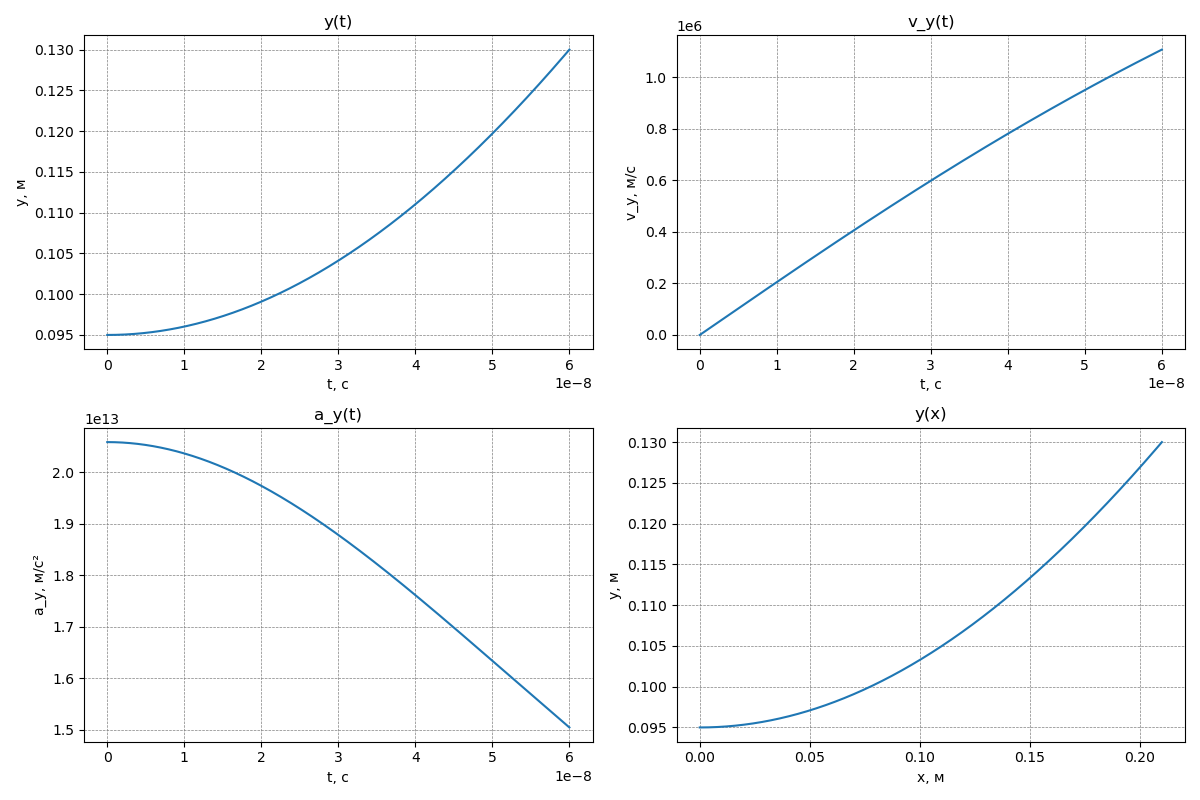
\includegraphics[scale=0.52]{mod2.png}


\large \textbf{Вывод} \normalsize

В итоге в ходе моделирования получили дифур решили с помощью scipy и метода бинарного поиска нашли минимальную разность потенциалов,
при которой электрон не вылетит из конденсатора. 
Также получили ответ $\Delta \varphi$ = 8.600117 В с точностью до 5 знака после запятой (задаю программно).
Также построили графики и получили время полета и конечную скорость электрона.


\end{document}